\documentclass[12pt,a4paper]{article}
\usepackage[T1]{fontenc}
\usepackage{layout}
\usepackage{geometry}
\usepackage{setspace}
\usepackage{graphicx}
\usepackage[skip=5pt plus1pt, indent=20pt]{parskip}

\graphicspath { {./img/} }
\setstretch{1.5}
\pagenumbering{gobble}

\renewcommand{\baselinestretch}{1.0}
\renewcommand{\figurename}{Gambar.}

\begin{document}

  \textbf{NAMA} : Radinal Shidiq Saragih

  \textbf{KELAS} : IF C 2023

  \textbf{NPM} : 5520123104

  \vspace {0.25cm}

    \begin{center}
      \section*{\textbf{Perbedaan ALU, CU, Register, Internal Bus,
      Sequencing Logic, Decoder, dan Kontrol Memori}}
    \end{center}

  \vspace {0.25cm}

  \begin{center}
    \subsection*{\textbf{ABSTRAK}}
  \end{center}

  Article ini bertujuan untuk melakukan perbandingan komponen internal
  dalam susunan sebuah Central Processing Unit (CPU) atau prosesor,
  serta beberapa konsep yang ada di organisasi CPU.

  Dengan menggunakan metode analisis, membandingkan fungsi dan kinerja
  masing-masing komponen. Analisis difokuskan untuk menemui perbedaan
  antara komponen dari segi fungsi dan kinerja.

  \begin{center}
    \subsection*{\textbf{PENDAHULUAN}}
  \end{center}

  \vspace {0.25cm}

      ALU, CU, Register, Internal Bus, Sequencing Logic, Decoder, dan Kontrol
      Memory adalah bagian-bagian internal yang penting dalam sebuah
      kinerja sistem komputer.

      Pemahaman dalam bagaimana konsep dan komponen di dalam organisasi CPU
      sangat penting untuk lebih memahami bagaimana sebuah CPU dapat berkerja
      dan alhasil bagaimana sebuah komputer bekerja.

  \begin{center}
    \subsection*{\textbf{METODE}}
  \end{center}

    Metode yang digunakan adalah metode analisis. Menganalisis bagaimana
    ALU, CU, Register, Internal Bus, Sequencing Logic, Decoder, dan Kontrol Memori
    bekerja serta peran apa yang dimilikinya di suatu arsitektur CPU.

    Dimulai dari deskripsi dari komponen-komponen CPU, dari deskripsi tersebut
    akan dilakukan identifikasi perbedaannya, kesamaan serta bagaimana
    mereka memiliki keterkaitan dengan satu sama lain.

  \begin{center}
    \subsection*{\textbf{PEMBAHASAN}}
  \end{center}

  \vspace {0.25cm}

    \begin{figure}[h]
      \centering
      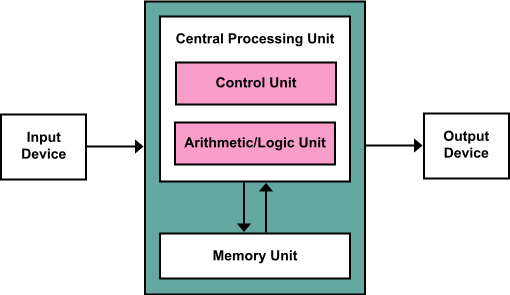
\includegraphics[scale=0.5]{CPUBASICDIAG}
      \caption{Diagram CPU}
      \label{fig:CPUBASICDIAG}
    \end{figure}

  \vspace {0.25cm}

    \subsubsection*{Register}

      Register, adalah tempat-tempat penyimpanan berukuran kecil namun
      berkecepatan tinggi yang terletak di unit memori CPU.

      Register sangat penting bagi CPU karena digunakan sebagai tempat dimana,
      operator, operand, atau pun hasil dari instruksi disimpan, sehingga
      dapat diakses dan operasikan.

    \subsubsection*{Internal Bus}

      Internal bus adalah hampir sama dengan konsep Sistem Bus,
      yaitu penghubung antara unit-unit yang terletak didalam suatu CPU,
      yaitu ALU, CU, ataupun Memory Unit.

      Jadi dengan adanya Internal Bus ini, unit-unit dalam CPU dapat berkomunikasi
      dengan satu sama lain dan berkerja secara harmonis.

    \subsubsection*{Arithmetic and Logical Unit (ALU)}

      ALU atau unit aritmatika dan logika atau boolean, unit ini berfungsi
      untuk memproses berbagai instruksi aritmatika dan logika yang
      disampaikan oleh unit control.

      Umumnya unit ini terdiri dari berbagai jenis gerbang logika
      (XOR, AND, OR, NOR, dll) sehingga unit akan memproses instuksi satu persatu
      dalam ukuran bit.

    \subsubsection*{Control Unit (CU), Sequencing Logic, Decoder, dan Kontrol Memori}

      Control Unit (CU), berfungsi untuk mengendalikan dan mengkoordinasikan
      seluruh kinerja sebuah prosessor atau CPU, mulai dari mengendalikan akses
      kepada memori, mengendalikan system bus, mengendalikan Unit Aritmatika dan
      logika atau ALU, sehingga mengendalikan bagaimana instruksi di proses.

      Decoder atau Unit Decoder, adalah bagian Control Unit yang berfungsi
      untuk memproses instuksi tersebut dan menghasilkan sinyal-sinyal kontrol
      yang sesuai.

      Secara teknis, Sequencing Logic mengacu kepada tahapan dimana suatu
      instruksi yang diproses oleh unit control akan di pastikan memiliki urutan
      eksekusi yang benar.

      Kontrol Memori, mengacu kepada Unit yang bertugas untuk pengendalian akses
      kepada memori, sama dengan decoder sebelumnya, unit ini umumnya ditemui
      di Unit Control.

      Penjelasan lebih lanjut apa saja bagian-bagian yang terdapat didalam
      Control Unit kita bisa sebagai berikut.

      \begin{itemize}

        \item \textbf{Control Lines}

          Sinyal-sinyal yang mengatur operasi dalam suatu unit pemrosesan, contohnya
          proses read/write atau untuk mengirim sinyal agar mengaktifkan ALU (Arith-
          metic Logic Unit).

        \item \textbf{ALU Control Unit}

          Bagian yang mengontrol operasi-operasi aritmatika yang dilakukan ALU (penam-
          bahan, pengurangan, perkalian, atau operasi logika).

        \item \textbf{Clock Circuit}

          Bagian yang mengatur alur waktu dalam pengeksekusian instruksi, agar diek-
          sekusi dengan urutan yang tepat.

        \item \textbf{Bus Interface Unit}

          Bagian yang berada diantara CPU dengan sistem bus komputer,
          merupakan dimana komunikasi antara sistem bus dan cpu terjadi.
          bagian inilah yang memberikan CPU akses ke komputer secara
          keseluruhan, seperti RAM, ataupun perangkat I/O.

        \item \textbf{Control Unit Sequencer}

          Bagian yang memastikan langkah-langkah instruksi memiliki urutan yang benar
          agar dapat dieksekusi dengan tepat atau tahap Sequencing Logic dalam
          pemrosesan instuksi.

        \item \textbf{Decoder}

          Bagian CPU yang menerima dan memproses atau decode instuksi yang diterima
          oleh Control Unit, sehingga dapat diartikan oleh control unit untuk
          mengendalikan eksekusi dan operasi di CPU.

        \item \textbf{Memory Control}

          Memory Control atau Kontrol Memori adalah unit yang berfungsi untuk
          mengendalikan segala hal yang bersangkutan dengan memori, seperti
          pembacaan dan penulisan data ke memori, pengelolaan alamat memori,
          dan koordinasi operasi-operasi memori lainnya.

      \end{itemize}


    \begin{center}
    \subsection*{KESIMPULAN}
    \end{center}

    Dari yang telah disampaikan diatas, pertanyaan "Perbedaan ALU, CU, Register, Internal Bus,
    Sequencing Logic, Decoder, dan Kontrol Memori" dapat kita simpulkan bahwa
    masing-masing bagian tersebut berbeda secara peran yang dimiliki didalam
    sistem komputer.

    Namun, meskipun berbeda dalam fungsi, semua bagaian yang dijelaskan diatas
    jika dalam suatu organisasi komputer, akan berkeja sama secara sinkronis
    dan sistematis sehingga komputer dapat berjalan sebagaimana seharusnya.

    \begin{center}
      \subsection*{DAFTAR PUSTAKA}
    \end{center}

      Architecture of the central processing unit (CPU). https://computersciencewiki.org/
  index.php/Architecture\_of\_the\_central\_processing\_unit\_(CPU), (diakses pada 20 Februari 2024).

      Patterson, David. A, dan Hennessy, John L.2012.Computer Organization and Design: The Hardware/Software Interface. Massachusetts:Morgan Kaufmann.

      Tanenbaum. Andrew S, dan Austin, Todd.2012.Structured Computer Organization.Michigan:Pearson.
\end{document}
